\subsection{Reactor Pattern}
\label{section:Reactor Pattern}

Das Reactor Pattern ist ein Design Pattern bei dem asynchrone auftretende Events, synchron abgearbeitet werden. Asynchron Nachrichten/Events werden vom Reactor Pattern in einen synchronen Programmfluss gebracht. Neben dem demultiplexen von asynchronen Nachrichten kann das Reactor Pattern verwendet werden um nicht blockierende I/O lastige Applikationen zu entwicklen. Da die Registrierung und der Aufruf von Ereignissen vom Reactor Pattern übernommen wird gibt es eine lose Koppelung zwischen dem lesenden und schreibenden I/O Operationen und der Business Logik der Applikation. \cite[p. 1]{Sch95}

\subsubsection{Motivation}
\label{section:reactor_motivation}

Douglas C. Schmidt beschreibt einen Anwendungsfall für das Reactor Pattern, bei dem Logging Informationen in einem Verteilten System an einen zentralen Server gesendet und gespeichert werden. Der Server soll in der Lage sein Logging informationen zu jederzeit speichern zu können. Dabei kann es vorkommen, dass Informationen auch von mehreren Clients gleichzeitig an den Server gesendet werden \cite[p. 1]{Sch95}. 

Eine Möglichkeit um mehrere Verbindungen auf einmal zu verarbeiten bietet Multithreading. Laut D. Schmit ist die Verwendung von Multithreading nicht unproblematisch, da folgende Probleme dabei auftreten können \cite[p. 1]{Sch95}: 

\begin{itemize}
  \item Benötigt ein komplexes concurrency Schema
  \item Auf Single Core Prozessoren kann es zu einer schlechten Performance kommen
  \item Es könnte nicht auf allen Betriebssystemen verfügbar sein.
\end{itemize}

Die Nachteile 2 und 3 können 20 Jahre nach dem erscheinen dieses Papers als hinfällig angesehen werden, da mittlerweile multicore Prozessoren im Consumer Bereich angekommen sind und jedes relevante Betriebssystem Threads unterstützt. Das Problem Nummer 1 mit dem komplexen concurrency Schema bei der Verwendung von Multithreading bleibt bis heute bestehen. Das Reactor Pattern wurde 1995 entwickelt und probiert alle drei dieser Probleme zu lösen indem es auf Multithreading verzichtet.

\subsubsection{Funktionsweise}

Das Reactor Pattern implementiert eine Event Loop welche sich um das versenden und empfangen von Events kümmert. Die Event Loop ist eine nicht endende Schleife, welche Events von außerhalb empfangen kann und dieser an den richtigen Empfänger weiterleiten kann. Um auf einen Ereignistyp reagieren zu können verwendet das Reactor Pattern Callback Funktionen, welche aufgerufen werden sobald ein Ereignis eintritt. Dadurch kann eine Applikation nur auf Ereignisse reagieren, für welche eine Callback Funktion verfügbar ist. Da das Reactor Pattern auf Multithreading verzichtet, kann immer nur eine Operation zu einem Zeitpunkt ausgeführt werden. I/O Operationen können jedoch gleichzeitig behandelt werden. In der Regel werden Callback Funktionen ausgeführt wenn eine blockierende I/O Operation abgeschlossen ist. Dabei können typische Ereignisse folgende sein \footnote{Die Liste ist angelehnt an folgenden Blog-Post: \url{http://pltconfusion.com/2014/10/20/eventmachine_internals_and_the_reactor_pattern/}}:

\begin{itemize}
  \item Eine Datei wurde von einem Filesystem gelesen
  \item Eine Datebank abfrage wurde gelesen
  \item Ein HTTP Request wurde kompletiert
\end{itemize}

Ob eine I/O Operation bereit abgeschlossen ist und dadurch nicht blockiert kann zum Beispiel über den Systemaufruf \emph{select} \footnote{Siehe auch Sektion \ref{section: Threads} Threads} bestimmt werden.

Der genaue Lebenszyklus des Reactor Patterns ist in Abbildung \ref{figure:reactor_cycle} beschrieben.

\begin{figure}[!htb]
  \centering
  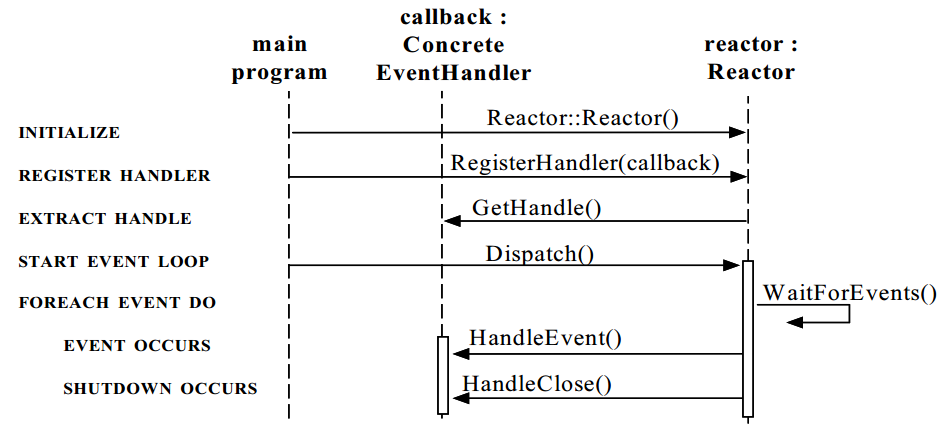
\includegraphics[width=13cm]{images/reactor.png}
  \caption{
    Zusammenarbeit der einzelnen Komponenten \cite[p. 5]{Sch95}
  }
  \label{figure:reactor_cycle}
\end{figure}

In der Initialisierung wird der Reactor in der \emph{main} Methode erstellt. Nachdem ein Reactor erstellt wurde können sich unterschiedliche \emph{Event Handler} beim Reactor registrieren. Ein \emph{Event Handler} ist eine Klasse welche auf ein bestimmtes Ereignis reagieren kann. Diese \emph{EventHandler} besitzten eine \emph{getHandler} Methode, welches die Callback Methode für ein Ereignis zurückliefert. Sind alle Handler beim Reactor Registriert startet die Eventloop und wartet auf Ereignisse. Sobald ein Event eintritt wird die Callback Methode ausgeführt. Im letzten Schritt wird der Handler geschlossen und die Eventloop wartet auf die nächsten Ereignisse. 

Wie genau die Eventloop einzelne Ereignisse behandelt variiert zwischen den einzelnen Implementierungen. Eine Mögliche Implementierung ist das Ereignis an das Ende einer Queue zu geben und bei jedem durchlauf der Eventloop wird genau ein Ergebnis von der Queue genommen und behandelt.

Der Ablauf welcher in Abbildung \ref{figure:reactor_cycle} beschrieben ist richtet sich sehr an statischen Programmiersprachen wie C++\footnote{In Kapitel \ref{section:implementation} wird das Reactor Pattern in Ruby Implementiert.}.

Durch die Verwendung des Reactor Patterns wird eine enge Koppelung zwischen unabhängigen Teilen der Applikation und Applikations abhängigen teilen gelöst. Dadurch werden die Tief liegenden und komplexen Componenten wie das Empfangen und Versenden von Events, von der EventLoop übernommen. Durch die Verwendung von Events für blockierende Operationen wird der Programmierfluss vereinfacht da keine synchronisation der Daten nötigt ist \cite[p. 2]{Sch95}

\subsubsection{Reactor - Design Pattern}

Im folgenden werden die einzelnen Komponenten des Reactor Patterns genauer untersucht. In Abbildung \ref{figure:reactor_otm} wird die OTM Notation verwendet \footnote[0]{OTM ist der vorgänger von UML nährer Informationen findet man unter: \url{http://www.uml.org/}}.

\begin{figure}[!htb]
  \centering
  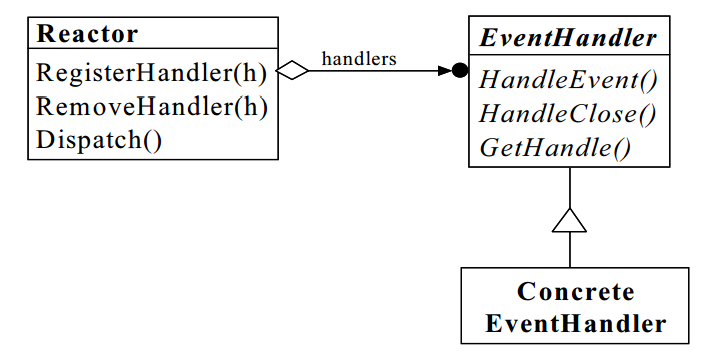
\includegraphics[width=9cm]{images/reactor_otm.png}
  \caption{
    Reactor OTM \cite[p. 4]{Sch95}
  }
  \label{figure:reactor_otm}
\end{figure}

\cite[p. 2]{Sch95}

\emph{Reactor:}
 Die Reactor Klasse ist für das registrieren, entfernen und versenden von Ereignissen verantwortlich. Die Eventloop, welche Callback Methoden von Ereignissen ausführt, befindet sich ebenfalls in dieser Klasse. Der Reactor ist Applikationsunabhängig und kann deswegen in anderen Applikationen wiederverwendet werden. 

\emph{Event Handler:}
Die Eventhandler Klasse bietet ein Interface für einen konkreten EventHandler. In dynamischen Sprachen wie Ruby oder JavaScript welche keine Interfaces bieten kann diese Klasse hinfällig sein. 

\emph{ConcreteEventHandler}
Der ConcreteEventHandler implementiert das Interface des Event Handlers. Dabei muss der Eventhandler folgende drei Methoden beinhalten: GetHandle, HandleEvent und StopEvent.

\subsubsection{Anwendungsgebiete}

Douglas Schmidt beschreibt in seiner Thesis folgende Anwendungsgebiete für das Reactor Pattern \cite[p. 4]{Sch95}:

\begin{itemize}
  \item Ein oder mehrere Ereignisse können gleichzeitig von unterschiedlichen Clients kommen
  \item Das Blockieren eines Clients oder das Pollen von Requests ist zu ineffizient
  \item Die gesendeten Nachrichten können in relativ kurzer Zeit verarbeitet werden
  \item Wenn unabhängige Teile der Applikation (Event Demultiplexing/Dispatching) von den abhängigen getrennt werden sollen
\end{itemize}

\subsubsection{Zusammenfassung}

Das Reactor Pattern bietet die Möglichkeit asynchron auftretende Ereignisse synchron abzuarbeiten. Durch den bewussten Verzicht auf Multithreading werden Probleme wie Deadlocks oder Race Conditions verhindert. Um dennoch mehrere Ereignisse gleichzeitig bearbeiten zu können, verwendet das Reactor Pattern eine bis zum Ende des Prozesses laufende Schleife. Diese Event Loop kümmert sich um das Empfangen und Versenden von Ereignissen. Dadurch werden asynchron auftretende Ereignisse wie sie bei einem Webserver auftreten können in einen synchronen Kontrollfluss gebracht. 

Das Reactor Pattern findet seine Einsatz in Applikationen welche durch viele blockierende I/O Operation abhängig sind. Durch die Verwendung des Reactor Patterns wird der Prozess nicht blockiert und somit in keinen Ruhezustand versetzt.